\documentclass[a4paper,12pt,twoside]{article}
\usepackage[polish]{babel}
\usepackage[utf8]{inputenc}
\usepackage[T1]{fontenc}
\usepackage{graphicx}
\usepackage{anysize}
\usepackage{enumerate}
\usepackage{fancyhdr}

\marginsize{4.5cm}{2.5cm}{2.5cm}{2.5cm}
\sloppy

\pagestyle{fancy}

\fancyhead{} 
\fancyhead[RO,LE]{\rightmark}
\fancyhead[LO,RE]{\leftmark}
\fancyfoot{} 
\fancyfoot[LE,RO]{Strona \thepage}
\fancyfoot[CO,CE]{***}
\renewcommand{\headrulewidth}{0.4pt}
\renewcommand{\footrulewidth}{0.4pt}



\title{Ptaki żyjące w Polsce}

\author{Ferdynand Wspaniały\\
\small Katedra Bocianoznawstwa\\
\small Uniwersytet Ornitologiczny w Krakowie\\
\small \texttt{ferdynand@uo.edu.pl}\\
}



\date{} %\date{02.03.2011}

\begin{document}

\maketitle

\tableofcontents

\begin{abstract}
Niniejszt artykuł o ptakach ma charakter popularny. Jego zadaniem jest szerzenie iedzy o skrzydlatych współmieszkańcach naszego kraju. Autor ma nadzieję, że przyczyni się ona do ukształtowania właściwego stosunku ludzi do żyjących u nas różnych gatunków ptaków. Wszystkie zawarte tu informacje pochodzą ze strony internetowej \texttt{http://ptaki.luzik.proste.pl}.
\end{abstract}

\section{Wprowadzenie}

Nauka zajmująca się badaniem i poznawaniem budowy organizmów ptaków oraz ich życia nosi nazwę ornitologii i jest częścią zoologii.\footnotetext{Przykładowy przypis} Do tej dyscypliny naukowej należy morfologia, tj. nauka o wyglądzie i budowie zewnętrznej i wewnętrznej ptaka, biologia - nauka o wszelkich przejawach ich życia fizycznego: ekologia, nauka o wymaganych przez dany gatunek warunkach środowiskowych oraz etologia - nauka o zwyczajach i sposobie zachowania się poszczególnych gatunków. W zakres wiedzy ornitologicznej wchodzi również systematyka zoologiczna, polegająca na podziale wszystkich ptaków na grupy systematyczne (gromada, rząd, rodzina, rodzaj, gatunek) według bliższego lub dalszego pokrewieństwa.

Niezależnie od systematyki przyjęto tutaj podział wszystkich ptaków na trzy grupy według ich użyteczności gospodarczej:
\begin{enumerate}[i)]
\item ptaki łowne, które w okresie lęgów znajdują się pod tzw. ochroną okresową,
\item ptaki objęte całoroczną ochroną, zwaną gatunkową,
\item ptaki, które w ciągu całego roku w ogóle nie podlegają ochronie.
\end{enumerate}
   

\section{Rodzina krukowatych}

\subsection{Kruk}

Stosunkowo nieliczny gatunek osiadły i zalatujący. Żyje w starych lasach, w pobliżu których znajdują się skaliste zbocza, poręby, łąki, miejsca rzadko odwiedzane. Gatunek monogamiczny łączący się w pary prawdopodobnie na całe życie. Okres gniazdowania: luty - kwiecień. Gniazda buduje z gałązek, umieszcza na drzewie lub na skale, samica wyściela je miękkim materiałem. Składa 4 - 6 zielonkawych jaj kształtu jajowatego z brązowymi plamami. Wysiaduje wyłącznie samica przez około 3 tygodnie; samiec ją w tym czasie żywi. Pisklęta są gniazdownikami, karmione przez obydwoje rodziców około 40 dni. 

\subsection{Gawron}

Pospolity gatunek osiadły i zalatujący. Przebywa najchętniej na terenach nizinnych w zagajnikach, alejach, parkach. Na terenach pagórkowatych występuje rzadko. W zimie stada gawronów pojawiają się w wielkich ilościach na polach oraz w osiedlach 'ludzkich, przeważnie są to osobniki z krajów położonych na północny wschód od Polski. Gnieździ się w koloniach na skrajach lasów, w zagajnikach i dużych parkach. Gniazdo umiejscawia na wysokich drzewach z dobrze rozwiniętą koroną. Jest ono dość niestarannie zbudowane z suchych gałązek trawy i suchych korzonków, wewnątrz wysłane sierścią. Gatunek monogamiczny. Okres gniazdowania: marzec - kwiecień. Samica znosi 3 - 5 jasnych, niebieskozielonych jaj, kształtu jajowatego, gęsto usianych żółtawymi i brązowymi plamkami. Jaja wysiaduje samica przez 18 - 19 dni. Pisklęta są gniazdownikami. Rodzice karmią młode przez 28-30 dni. 

\section{Rodzina jaskółkowatych}

\subsection{Jaskółka dymówka}

Pospolity ptak lęgowy i przelotny. Przylatuje w połowie kwietnia, odlatuje od sierpnia do września, czasem dopiero w październiku. Żyje w mniejszych miastach i na wsiach, unika większych miast. Gnieździ się w budynkach, najchętniej w stajniach i oborach, pod dachem. Gniazdo ma kształt miskowaty, zbudowane jest z gliny i źdźbeł trawy zmieszanych ze śliną. Wnętrze wysłane jest pierzem i sierścią. Gatunek monogamiczny. Gniazduje dwa razy w roku - w maju i w czerwcu. Znosi 4 - 6 białych jaj kształtu jajowatego z fioletowoszarymi i brązowoczerwonymi plamkami. Wysiadywanie trwa 14 - 16 dni. Pisklęta są rzekomymi gniazdownikami, legną się okryte białawym puchem. Wykarmianie piskląt trwa około 24 dni. 

\subsection{Jaskółka oknówka}

Liczny gatunek lęgowy i przelotny. Przylatuje w kwietniu, odlatuje we wrześniu. Przebywa w miejscach, w których żyje również jaskółka dymówka. Gniazdo buduje pod dachami budynków, rzadziej gnieździ się wewnątrz budynku. Gniazdo jest ulepione z gliny zmieszanej z błotem i śliną, w kształcie ćwierć kuli przyczepionej pod okapem dachu do ściany. Wewnątrz wysłane jest pierzem i sierścią. Gatunek monogamiczny. Gniazduje dwa razy w ciągu roku. Znosi 4 - 5 czystobiałych jaj, kształtu jajowatego. Wysiaduje samiczka i samiec przez około dwa tygodnie. Pisklęta karmione przez 21 - 23 dni, są rzekomymi gniazdownikami, lęgną się okryte białawym puchem. 

\begin{figure}
\centerline{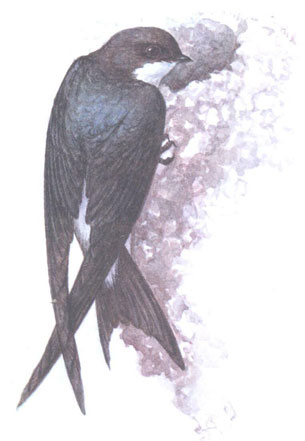
\includegraphics[scale=0.5]{jaskolka-oknowka}}
\caption{Jaskółka oknówka}
\end{figure}

\section{Rodzina bażantowatych}

\subsection{Bażant łowny}

Jest ptakiem łownym pod ochroną okresową -- koguty od 01.03 do 30.09, kury cały rok z wyjątkiem ośrodków hodowlanych, gdzie ochrona obowiązuje od 01 02 do 30.09.
Na rysunku~\ref{fig:bazant} z lewej strony samica (kura) z prawej samiec (kogut). 

\begin{figure}
\centerline{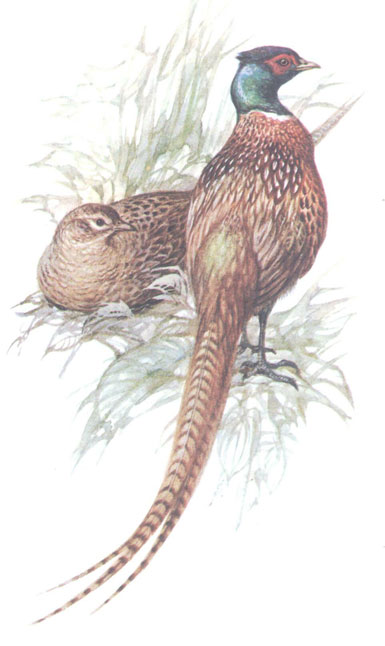
\includegraphics[scale=0.5]{bazant-lowny}}
\caption{Bażant łowny}
\label{fig:bazant}
\end{figure}

Bażanty nie posiadają jednakowego ubarwienia. Poprzez krzyżowanie kilku gatunków wytworzyły się u kogutów różnice w kolorze upierzenia. Podstawowym jego kolorem jest miedziany z ciemnymi poprzecznymi pasami. Kura jest popielatobrązowa z ciemniejszymi pasami. Młode ptaki są podobne do samicy. Kogut ma szyję najczęściej niebieskofioletową z zielonym połyskiem, wokół niej występuje biały pierścień. Dookoła oczu czerwona obwódka.

Ulubionym środowiskiem bażanta są pola i łąki sąsiadujące z gęstymi zaroślami. Zimą przebywa najchętniej w okolicy stogów i siedzib ludzkich. Jest ceniony jako ptak łowny oraz jako niszczyciel szkodników. Jest ptakiem-włóczęgą, niechętnie przebywa w jednym miejscu. Gatunek osiadły, poligamiczny. Gniazdowanie trwa przez całą wiosnę. Tokuje od kwietnia do końca maja. W tym czasie wokół niego gromadzą się kury. Na początku maja kura znosi do dołka ukrytego w zaroślach 6-18 jaj, kształtu jajowatego, koloru brudnojasnooliwkowego. Wysiaduje 24-26 dni. Pisklęta są zagniazdownikami. Samica opiekuje się nimi przez cały rok. 


\subsection{Kuropatwa}

Jest ptakiem łownym pod ochroną okresową od 22. 10 do 10.09.
Na rysunku~\ref{fig:kuropatwa} pokazano samca (koguta). 

\begin{figure}
\centerline{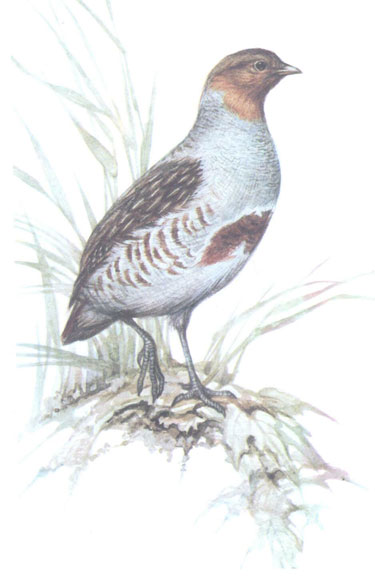
\includegraphics[scale=0.5]{kuropatwa}}
\caption{Kuropatwa}
\label{fig:kuropatwa}
\end{figure}

Samiec niewiele różni się od samicy. Obydwa ptaki są rdzawo brązowe, strona spodnia ciała popielatoniebieska. Samiec ma na piersi ciemnobrązową podkowę, której u samicy brak lub jest słabo zaznaczona. Dorosłe kuropatwy mają popielate nogi, młode zaś - żółte lub żółtopopielate.

Gatunek osiadły, pospolity w całym kraju. Bytuje na nizinach i terenach pagórkowatych. Najchętniej przebywa na polach uprawnych. Wiosną w porze lęgowej żyje w parach, w ciągu lata cała rodzina jest razem. W zimie kuropatwy skupiają się w stada. Kuropatwa niechętnie opuszcza miejsce gniazdowania, chyba że jest zmuszona w zimie szukać pożywienia, wraca jednak na stare miejsce. Jest cenna, gdyż skutecznie niszczy szkodniki w rolnictwie oraz jest ptakiem łownym. Gniazdowanie: kwiecień - czerwiec. Jest gatunkiem monogamicznym. Łączy się w pary na okres roczny. Znosi na wiosnę 10-20 żółtopopielatych, czasem czerwonawych lub zielonawych jaj, kształtu jajowatego. Gniazdo ukrywa na polu w koniczynie, lucernie, w zbożu itp. W przypadku zniszczenia zniesienia kuropatwa składa nowe. Wysiadują oboje rodzice 21-23 dni. Pisklęta są zagniazdownikami. 


\end{document}
